\subsection{Backend}
Il backend di BugBoard26 è sviluppato in Java con il framework Spring Boot e segue un'architettura a livelli (layered architecture). Il codice è suddiviso nei seguenti package:

\needspace{10\baselineskip}
\subsubsection{Package config}
Qui si trovano le classi di configurazione. La classe \texttt{SecurityConfig} definisce il \texttt{PasswordEncoder} con BCrypt, mentre \texttt{WebSecurityConfig} configura la catena di filtri HTTP con autenticazione Basic, le policy CORS per le richieste dal frontend e le regole di autorizzazione basate sui ruoli (ad esempio, solo gli amministratori possono creare o eliminare utenti).

\begin{figure}[H]
    \centering
    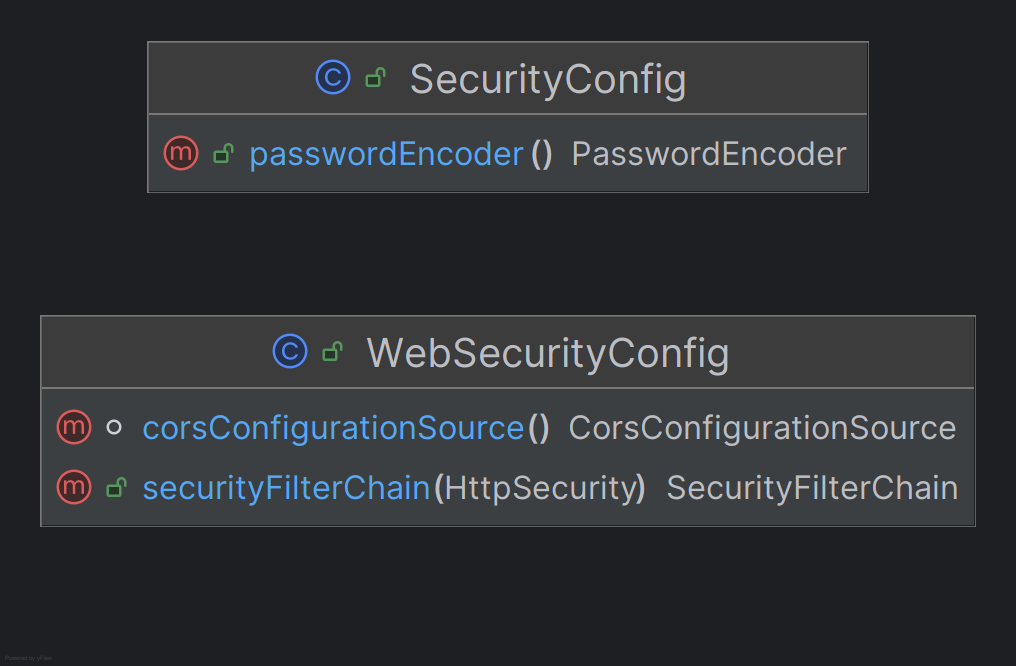
\includegraphics[width=0.6\textwidth]{package config.png}
    \caption{Package diagram del package config}
\end{figure}

\needspace{10\baselineskip}
\subsubsection{Package controller}
Raccoglie i controller REST che espongono le API. Ogni controller corrisponde a una risorsa (utenti, progetti, issue, commenti, allegati, etichette, notifiche) e definisce gli endpoint HTTP (GET, POST, PUT, DELETE) per le operazioni CRUD. Il \texttt{SseController} gestisce le connessioni Server-Sent Events per le notifiche in tempo reale.

\begin{figure}[H]
    \centering
    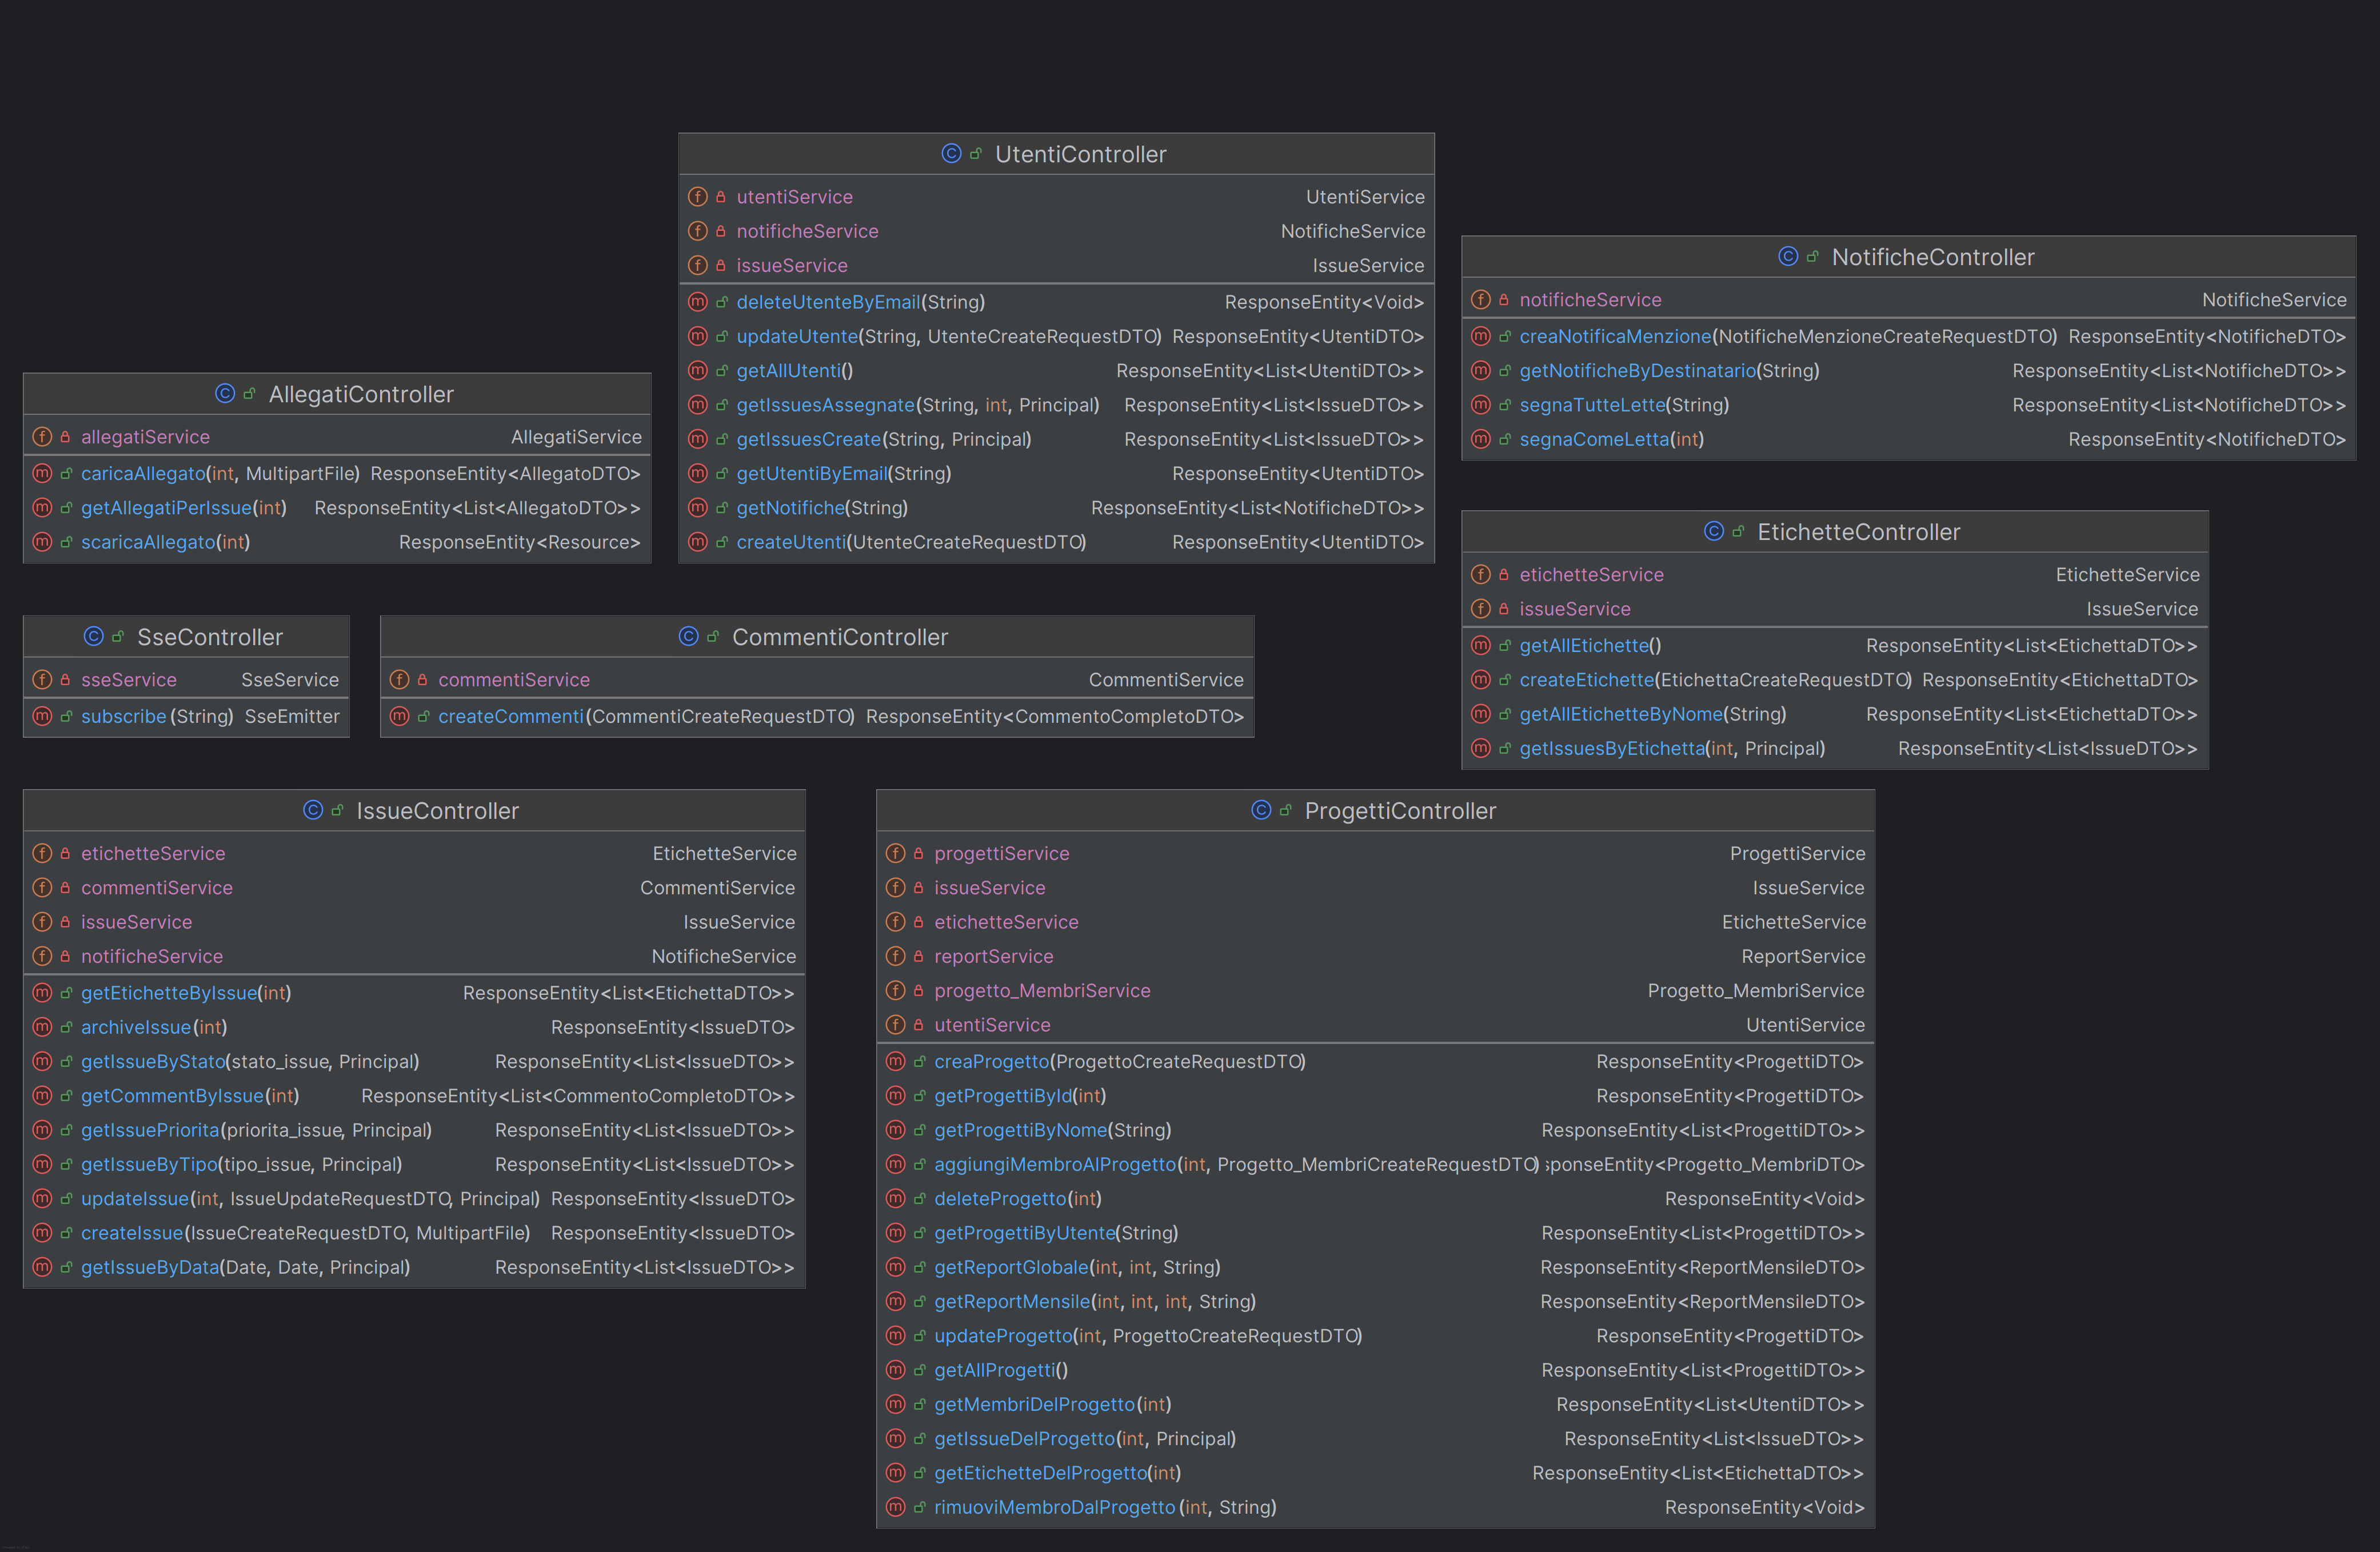
\includegraphics[width=1\textwidth]{package controller.png}
    \caption{Package diagram del package controller}
\end{figure}

\needspace{10\baselineskip}
\subsubsection{Package dto}
Raccoglie i Data Transfer Object (DTO), ovvero classi usate per trasferire dati tra frontend e backend senza esporre direttamente le entità del database. Ci sono DTO di risposta (es.\ \texttt{IssueDTO}, \texttt{UtentiDTO}), DTO di richiesta (es.\ \texttt{IssueCreateRequestDTO}, \texttt{IssueUpdateRequestDTO}) e DTO per i report (\texttt{ReportDTO}, \texttt{ReportMensileDTO}, \texttt{ReportUtenteDTO}).

\begin{figure}[H]
    \centering
    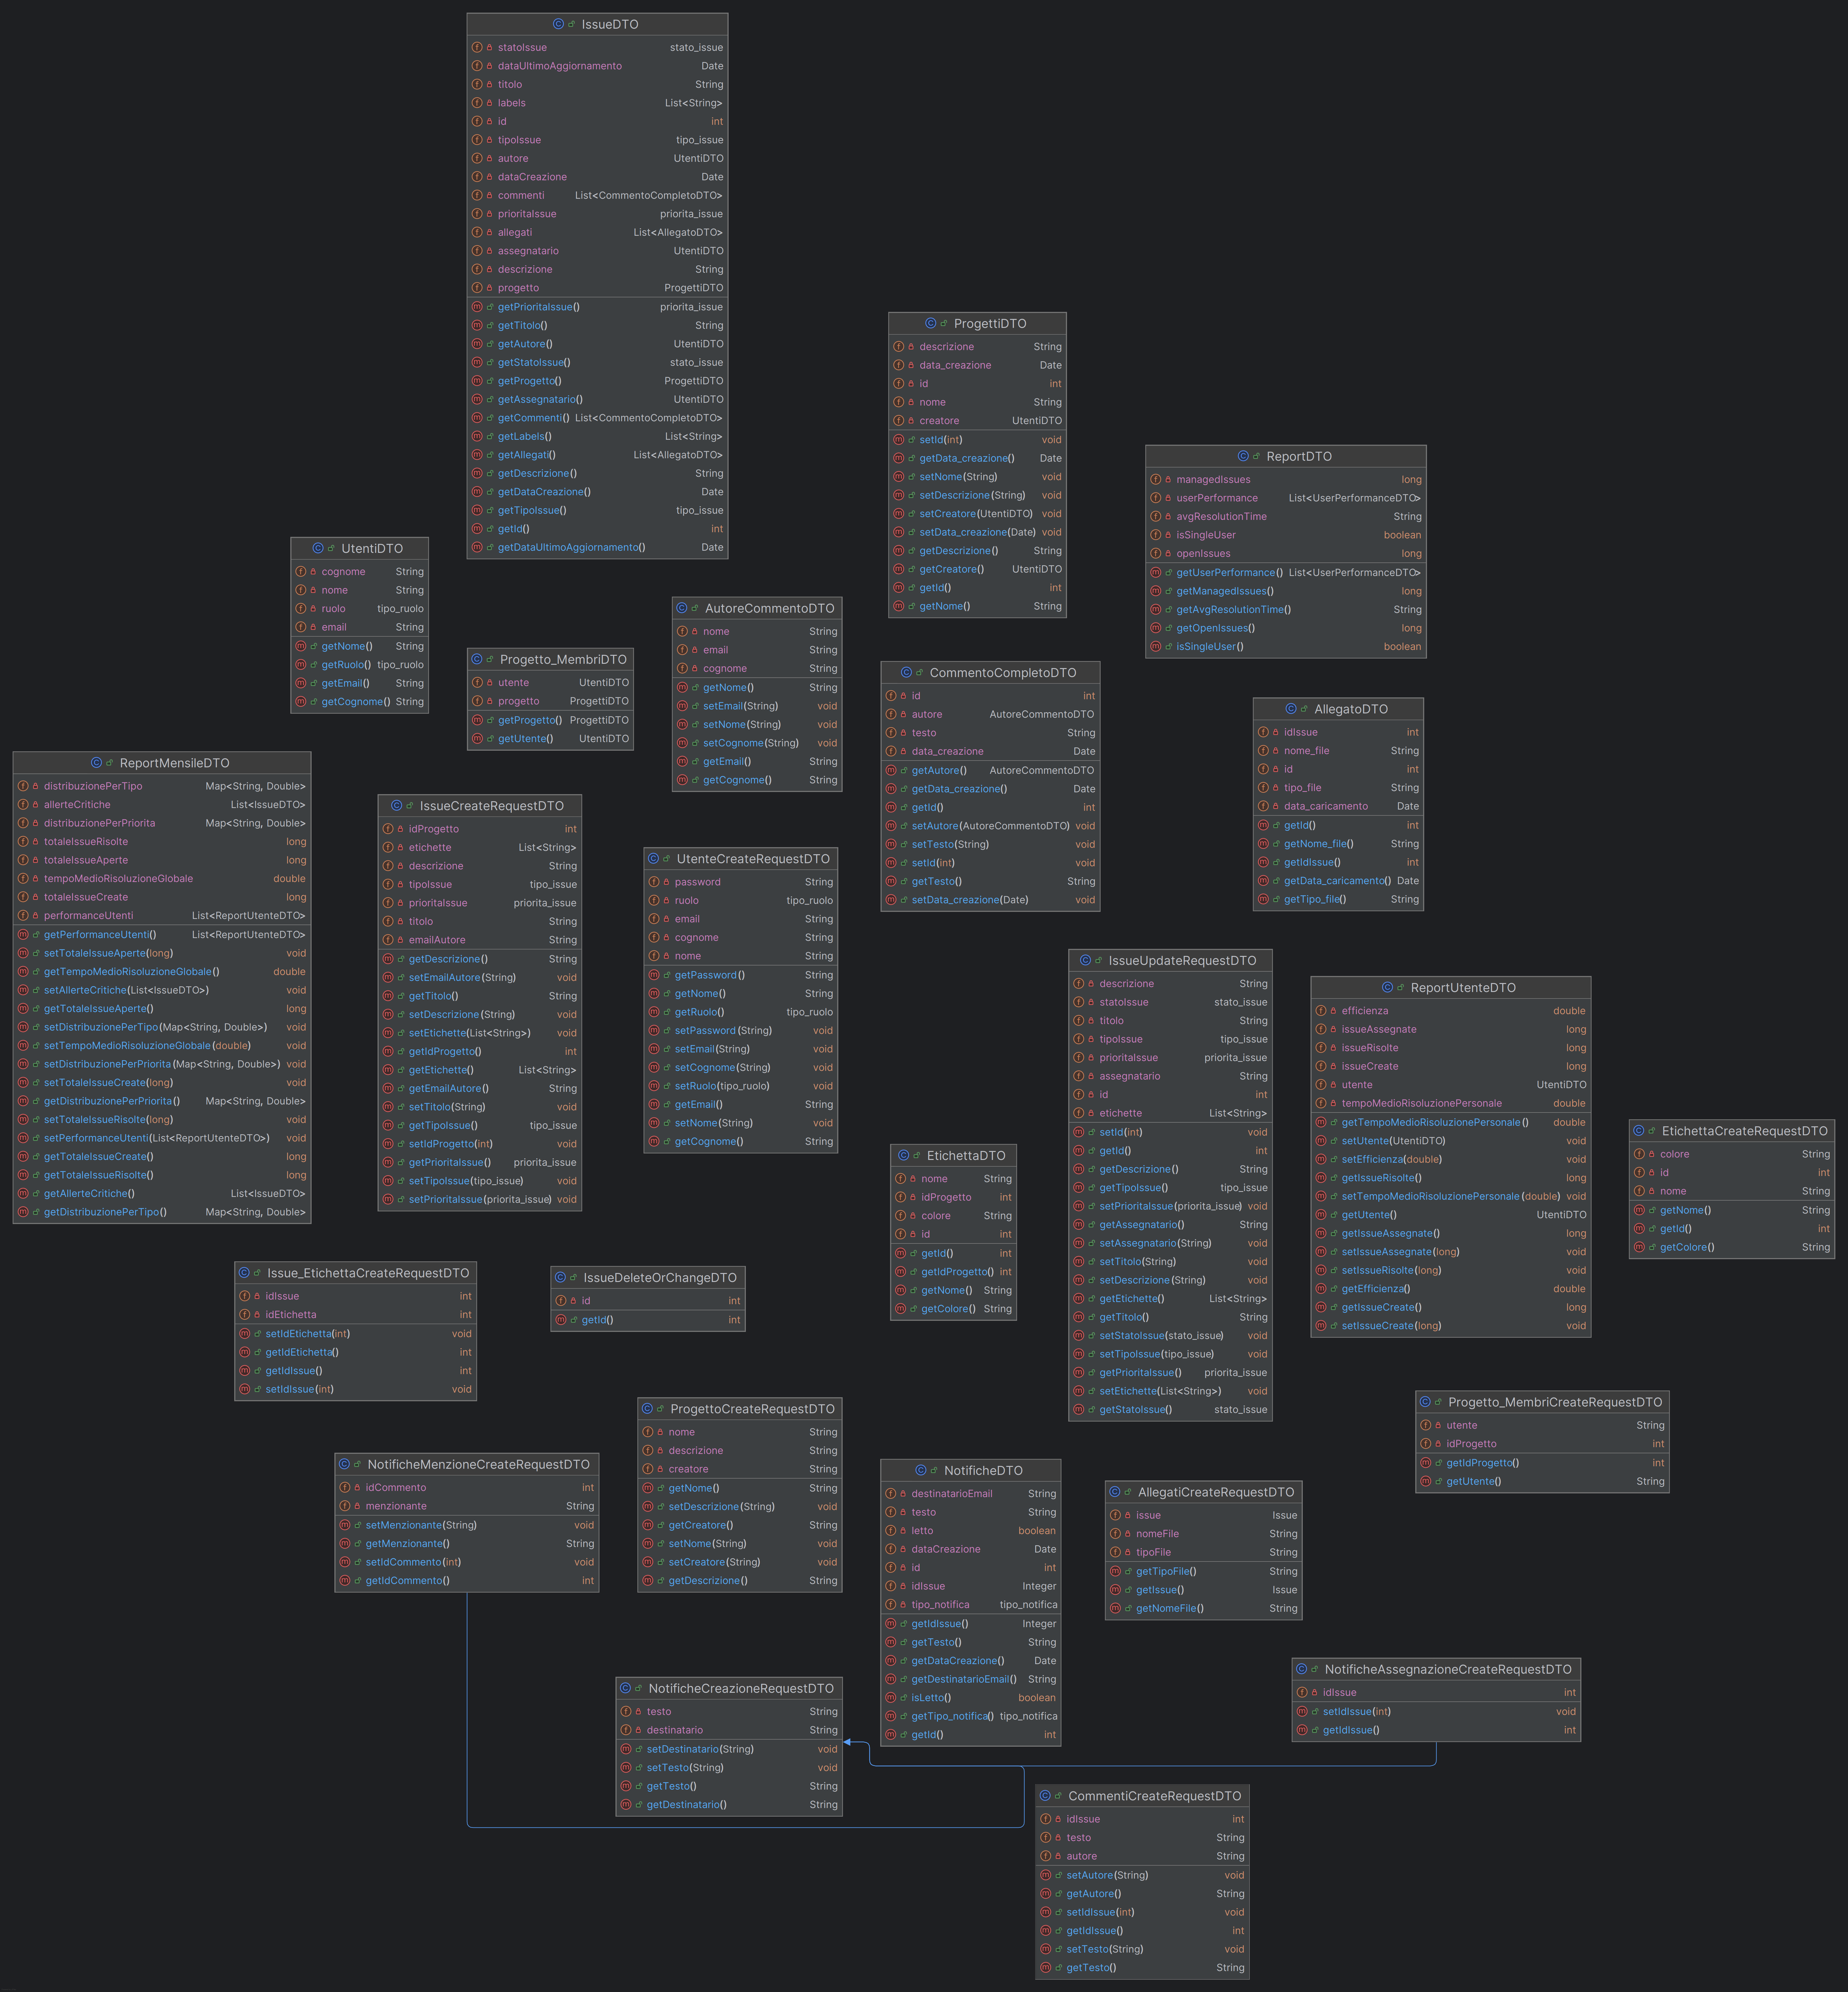
\includegraphics[width=1\textwidth]{package dto.png}
    \caption{Package diagram del package dto}
\end{figure}

\needspace{10\baselineskip}
\subsubsection{Package entity}
Qui ci sono le entità JPA che mappano le tabelle del database. Ogni classe corrisponde a una tabella (es.\ \texttt{Issue}, \texttt{Utenti}, \texttt{Progetti}) con campi, relazioni e vincoli definiti tramite annotazioni JPA. Il sotto-package \texttt{ComposedPrimaryKeys} contiene le chiavi primarie composite (es.\ \texttt{Issue\_EtichettePrimaryKey}, \texttt{Progetto\_MembriPrimaryKey}), mentre \texttt{enumerations} contiene i tipi enumerativi (\texttt{priorita\_issue}, \texttt{stato\_issue}, \texttt{tipo\_issue}, \texttt{tipo\_notifica}, \texttt{tipo\_ruolo}).

\begin{figure}[H]
    \centering
    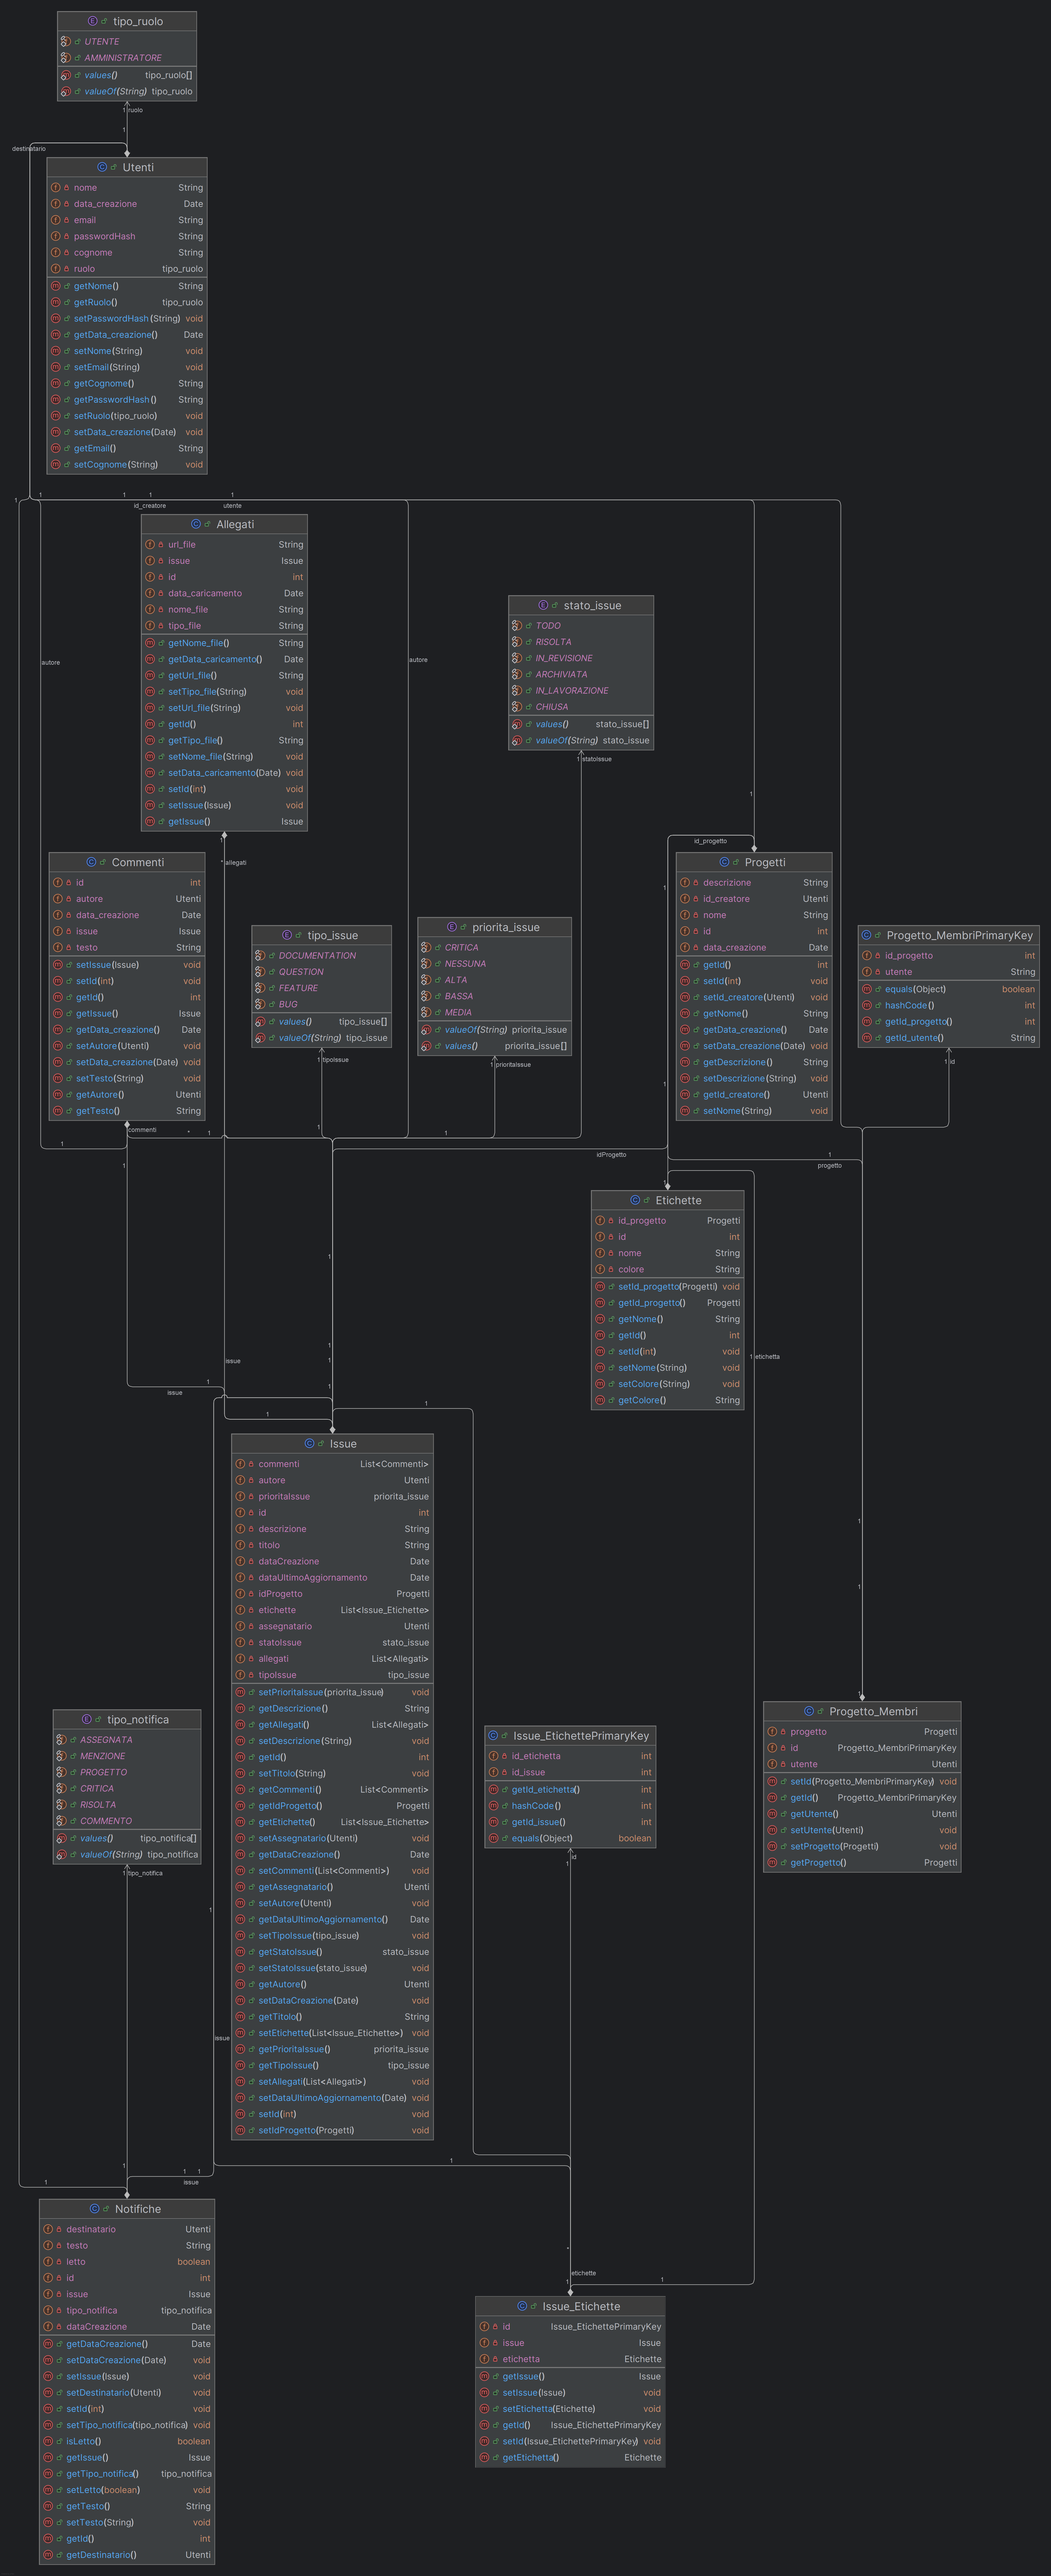
\includegraphics[width=0.5\textwidth]{package entity.png}
    \caption{Package diagram del package entity}
\end{figure}

\needspace{10\baselineskip}
\subsubsection{Package exception}
Contiene le classi per la gestione degli errori e le eccezioni personalizzate (come \texttt{ResourceNotFoundException} o \texttt{BadRequestException}). Invece di far gestire i problemi ai singoli componenti, la classe \texttt{GlobalExceptionHandler} cattura le eccezioni a livello globale e le converte in risposte HTTP standardizzate e coerenti per il frontend.

\begin{figure}[H]
    \centering
    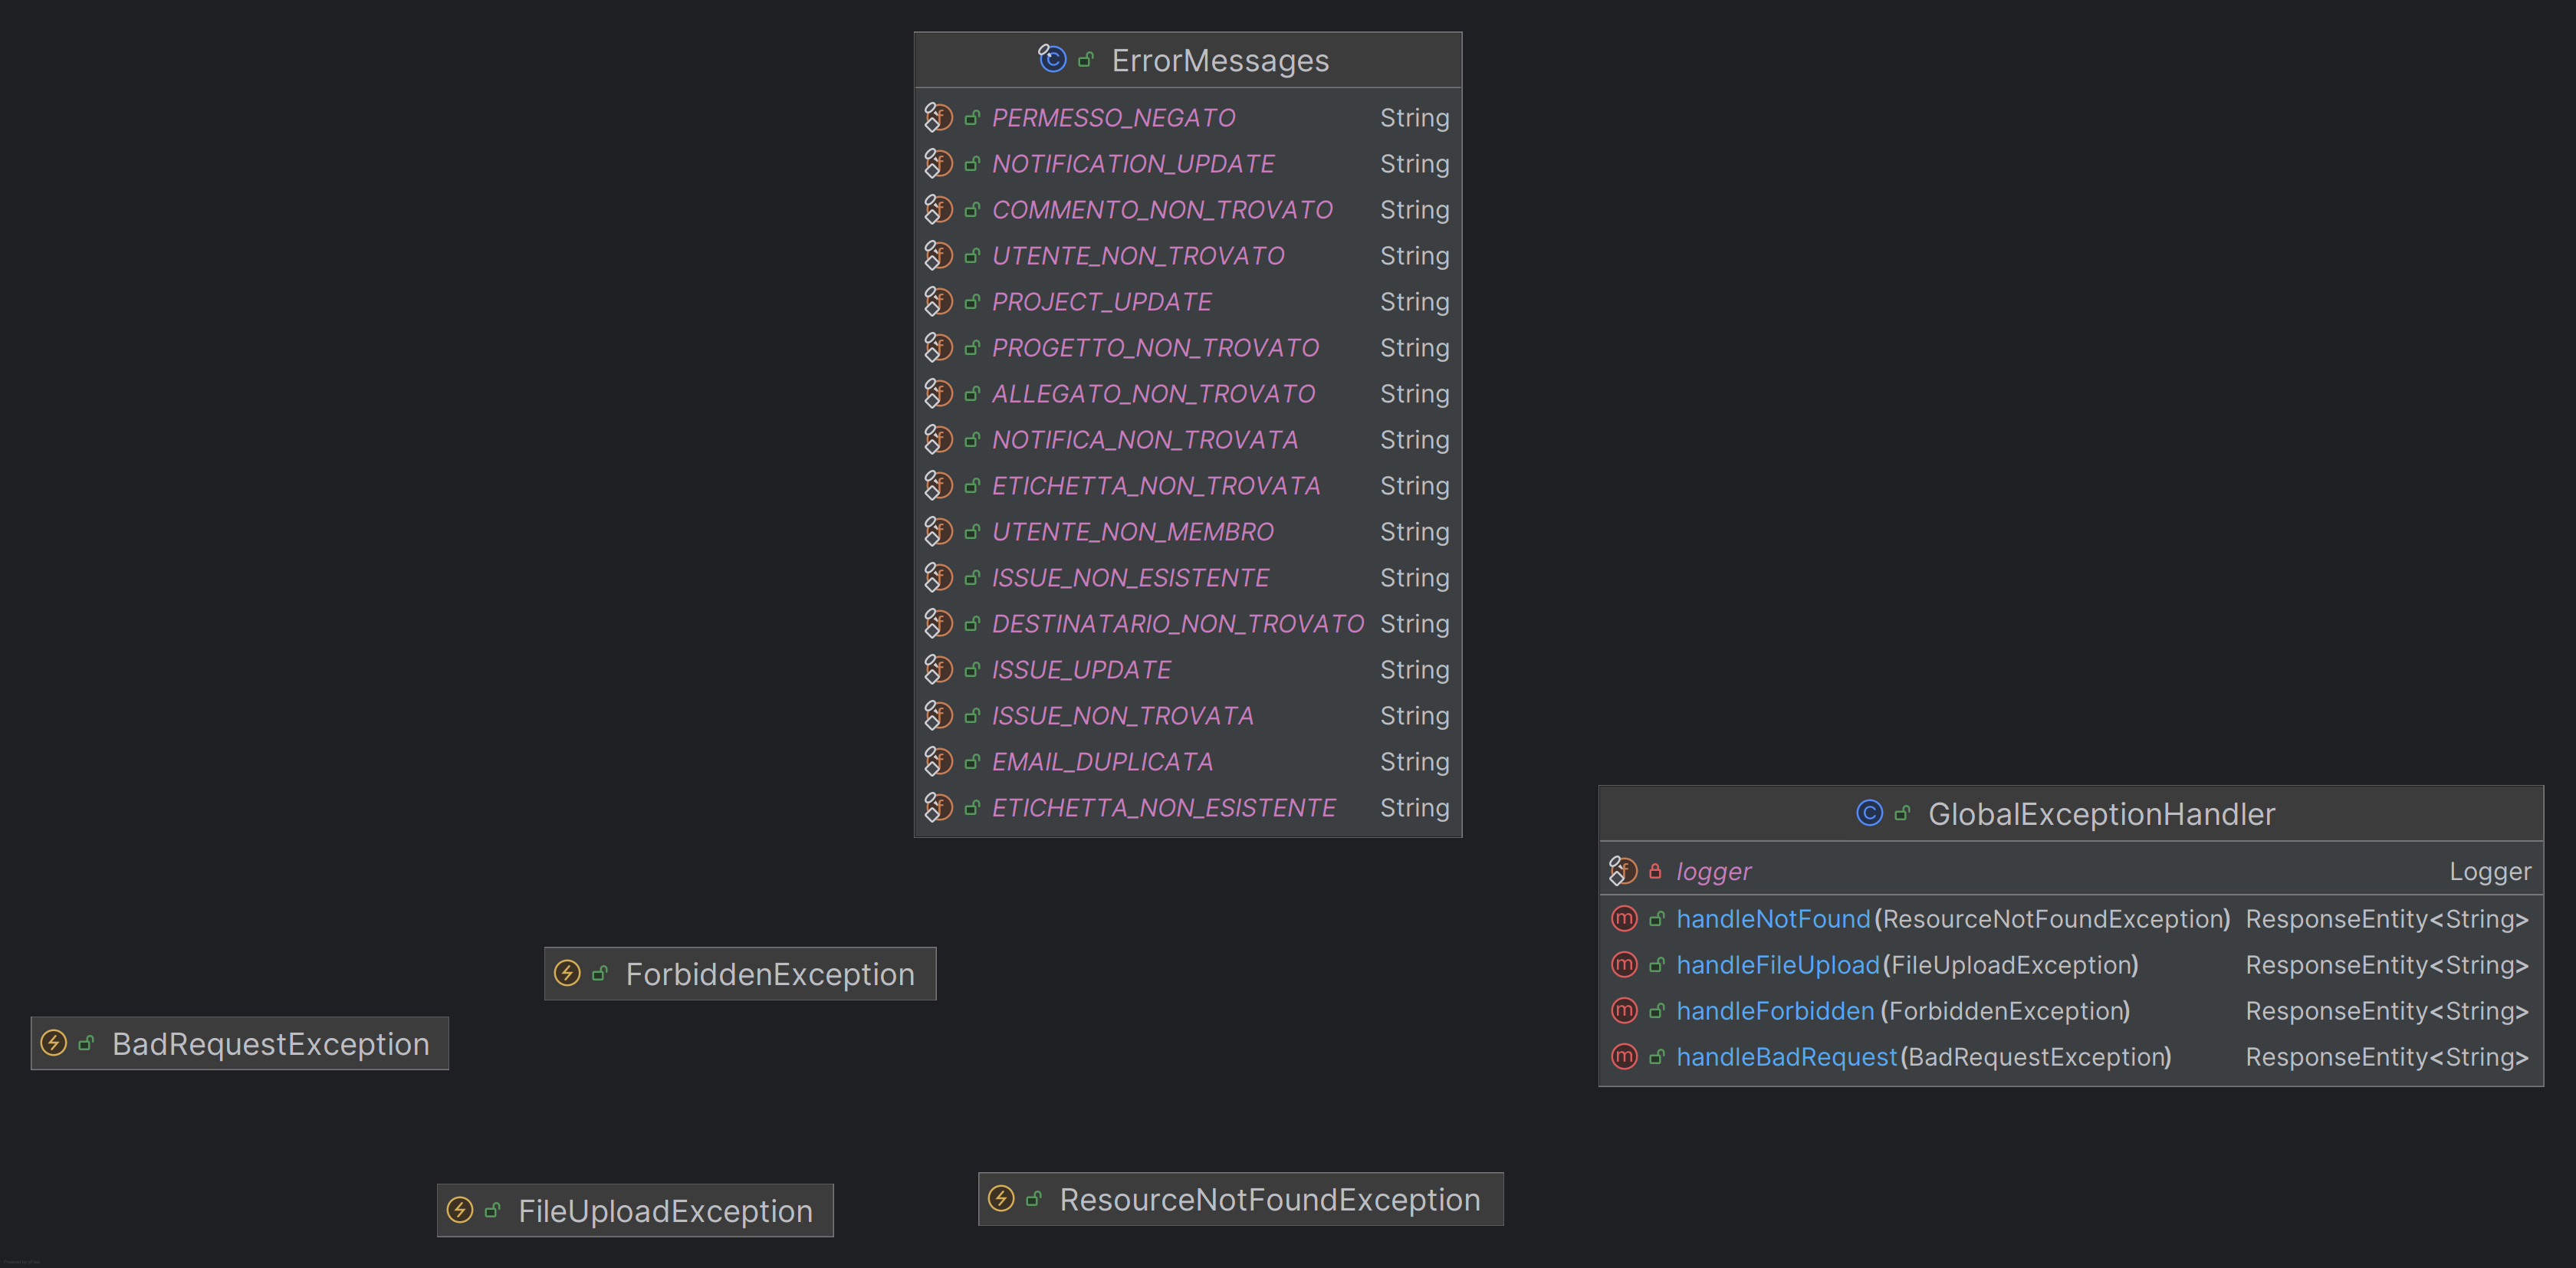
\includegraphics[width=0.8\textwidth]{package extensions.png}
    \caption{Package diagram del package exception}
\end{figure}

\needspace{10\baselineskip}
\subsubsection{Package repository}
Raccoglie le interfacce repository che estendono \texttt{JpaRepository} di Spring Data JPA. Ogni repository è legato a un'entità e fornisce i metodi per l'accesso ai dati, sia query CRUD predefinite che query personalizzate. C'è un repository per ogni entità: utenti, progetti, membri dei progetti, issue, etichette, associazioni issue-etichette, commenti, allegati e notifiche.

\begin{figure}[H]
    \centering
    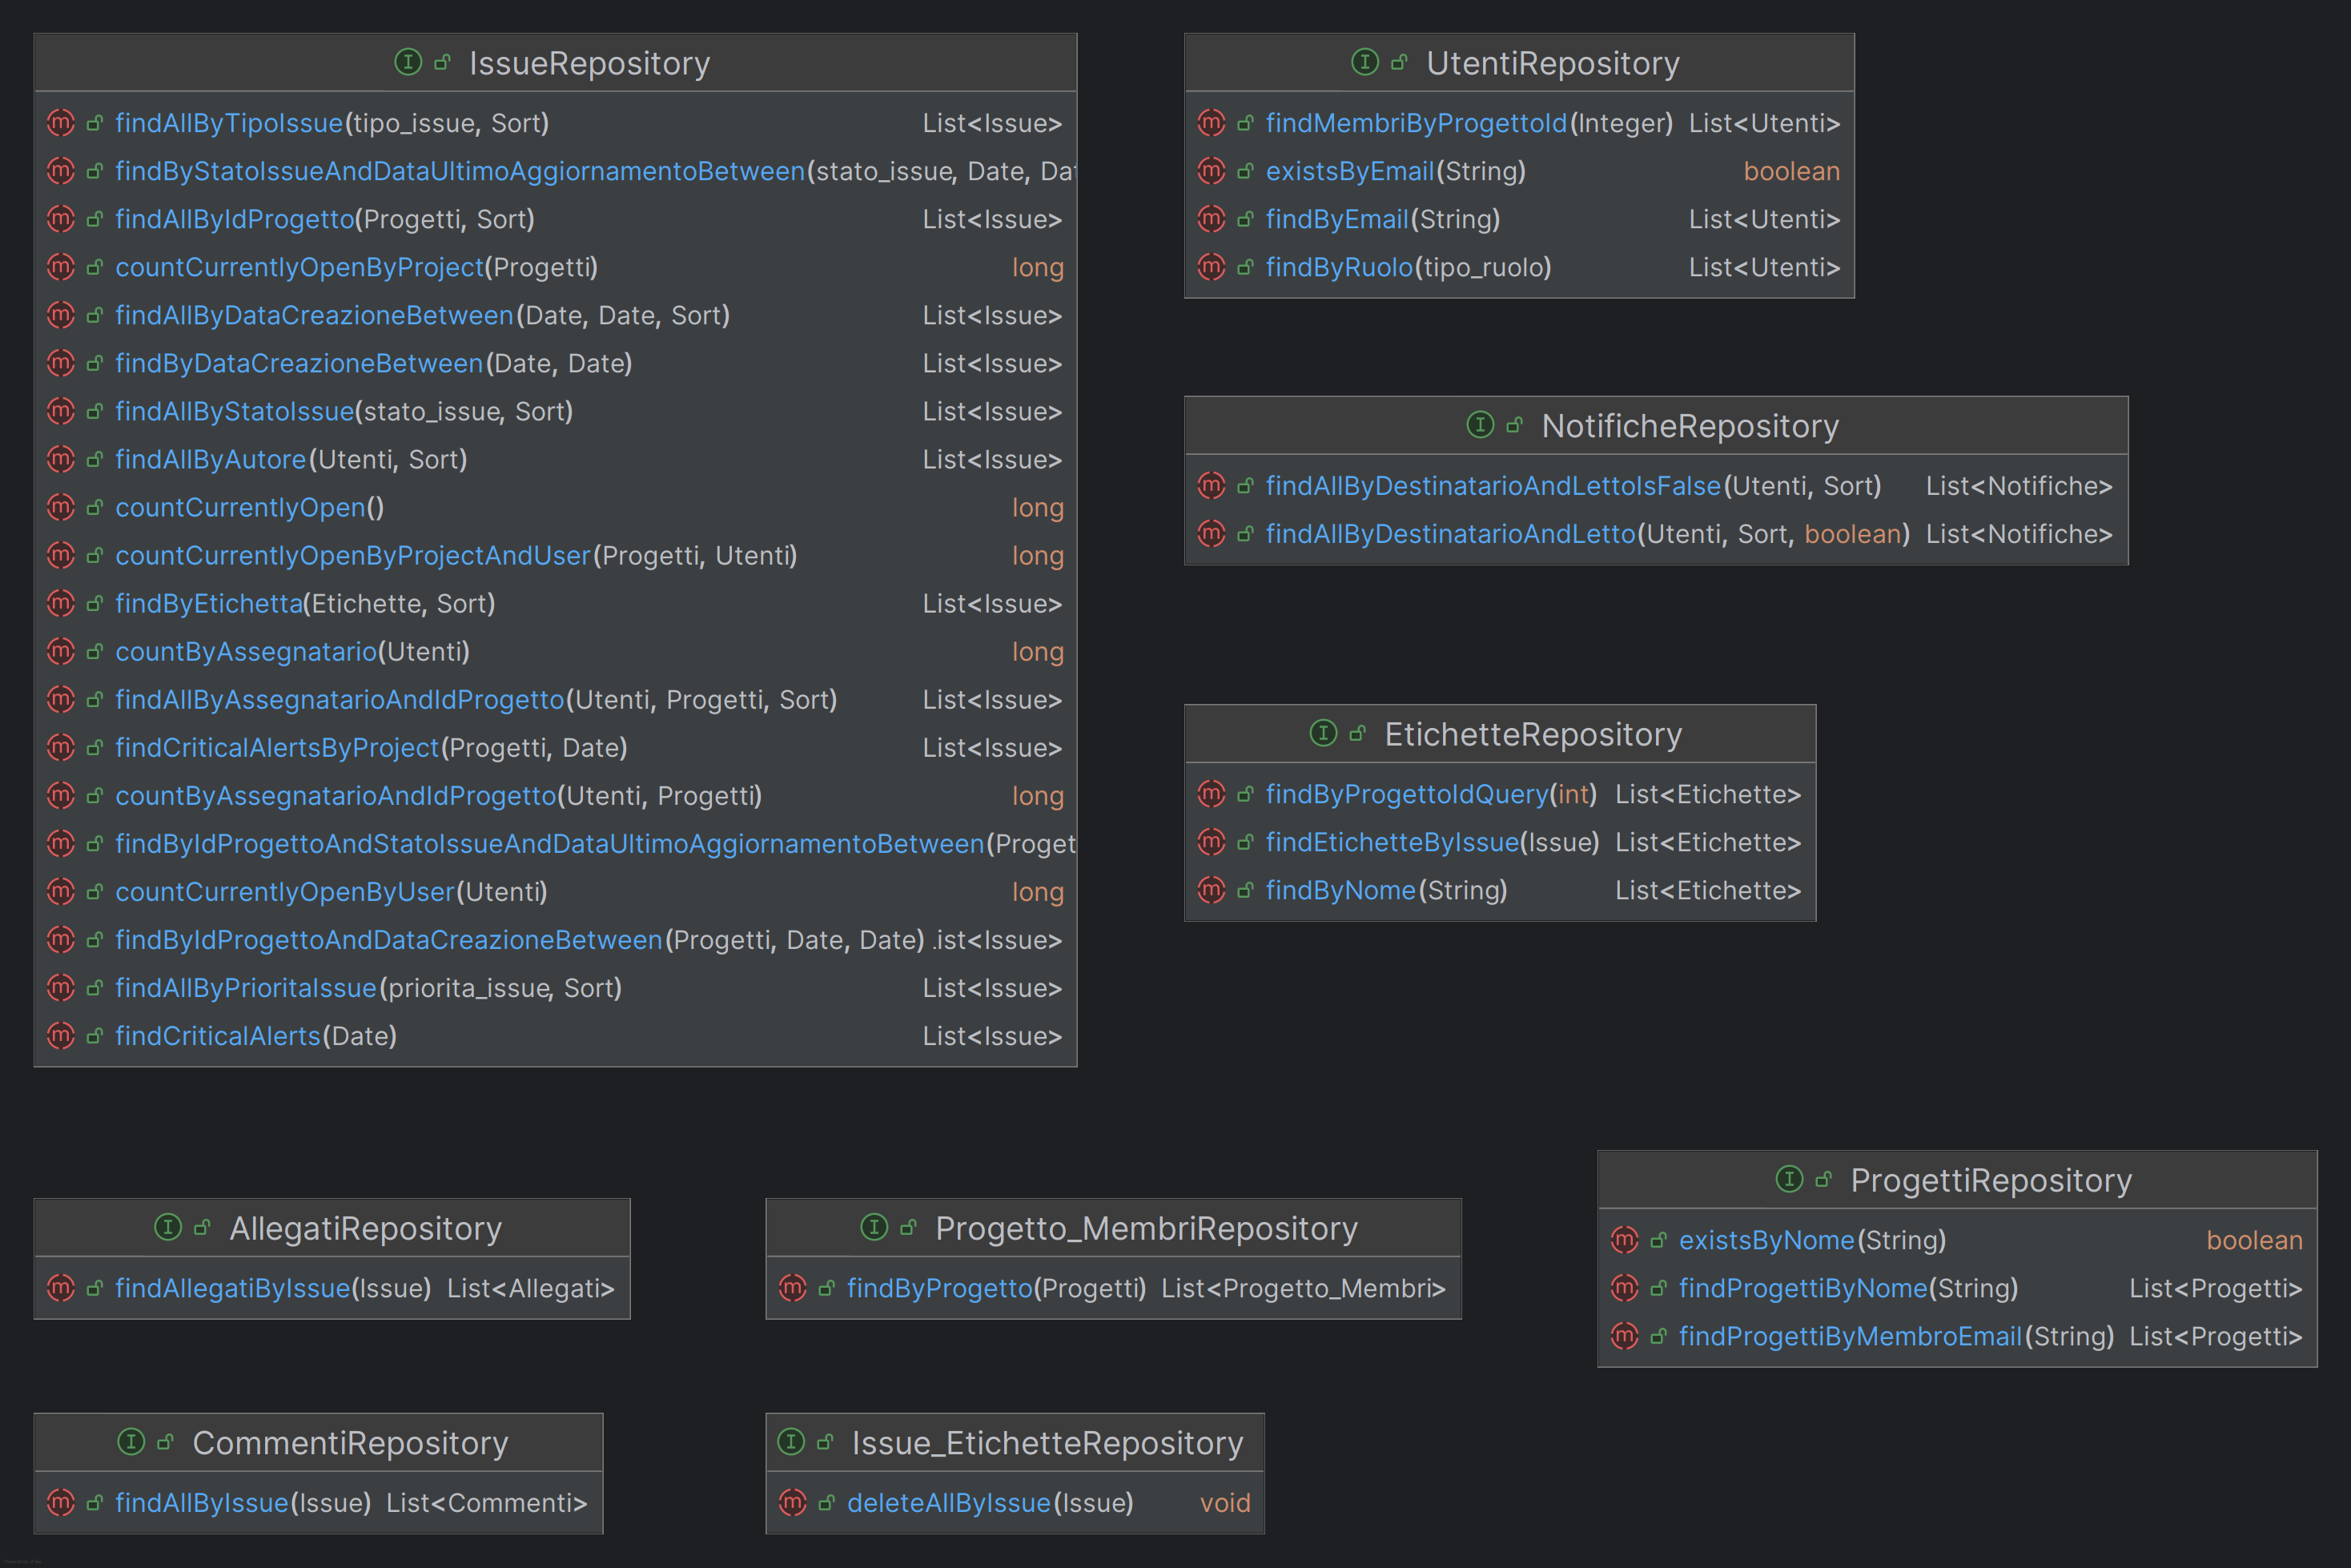
\includegraphics[width=1\textwidth]{package repository.png}
    \caption{Package diagram del package repository}
\end{figure}

\newpage
\subsubsection{Package service}
Raccoglie le classi di servizio con la logica di business. Ogni service si interpone tra il controller e il repository, occupandosi della validazione dei dati, delle trasformazioni tra entità e DTO, e delle operazioni che coinvolgono più entità. Il \texttt{SseService} gestisce le notifiche in tempo reale tramite Server-Sent Events, mentre il \texttt{ReportService} si occupa della generazione di statistiche.

\begin{figure}[H]
    \centering
    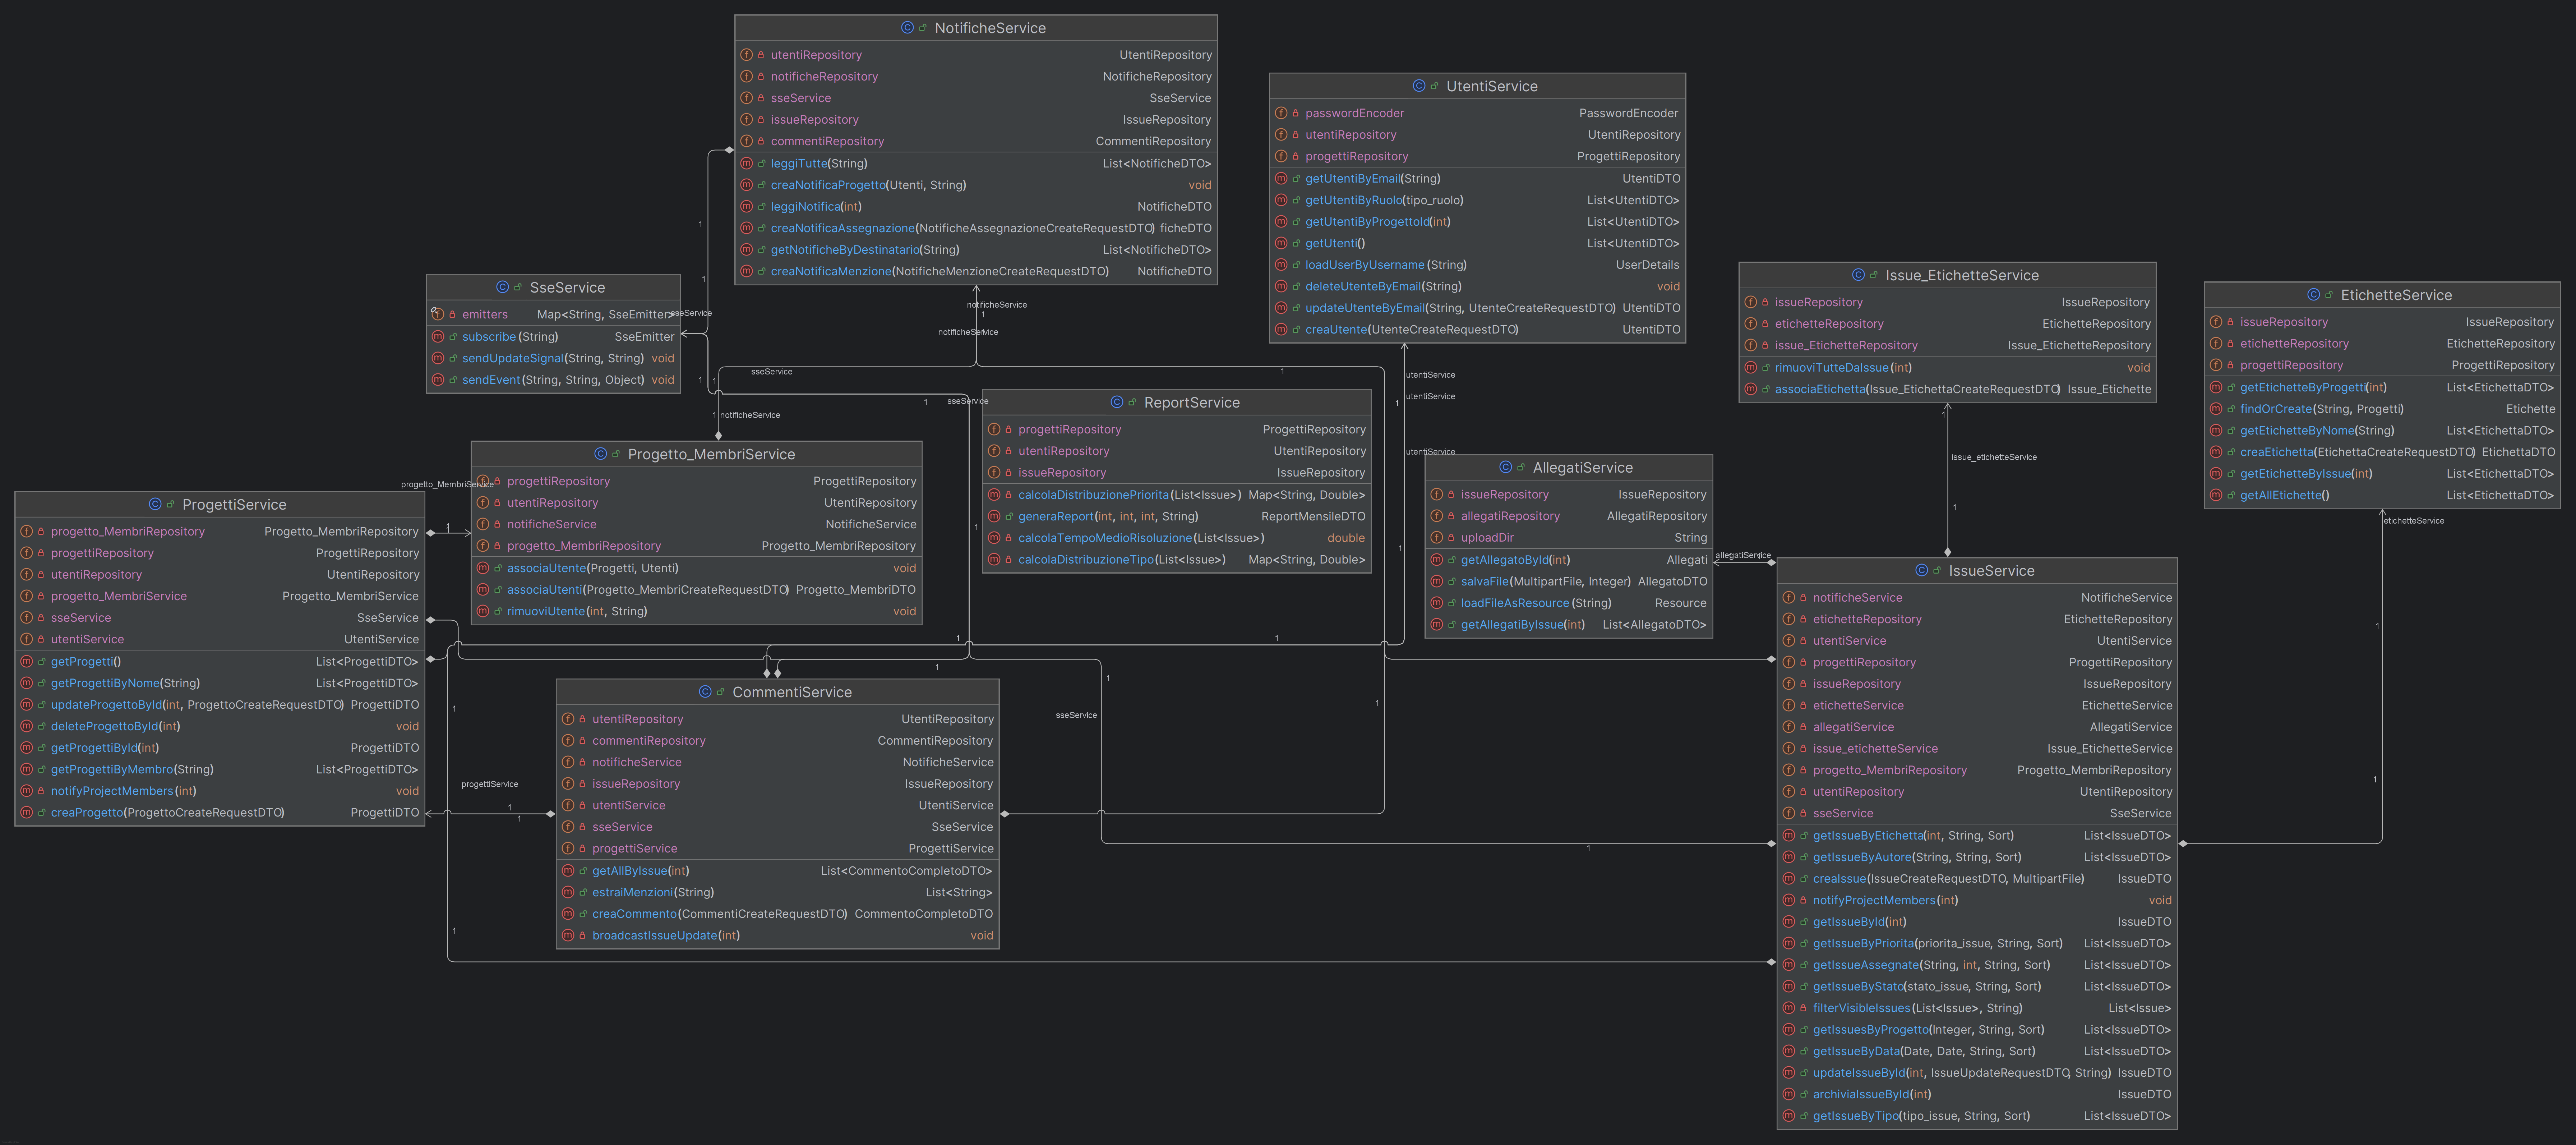
\includegraphics[width=1\textwidth]{package service.png}
    \caption{Package diagram del package service}
\end{figure}
\newpage

\subsection{Frontend}

Anche se nel diagramma utilizziamo una notazione simile alle classi, il frontend in React è costruito quasi esclusivamente con componenti funzionali. Il codice è organizzato per tenere ben separate la grafica dalla pura logica. I componenti visivi sono divisi per area funzionale (le issue, i progetti, o gli utenti) ed esistono poi librerie di elementi base condivisi (come bottoni, finestre modali o il layout generale).

Per evitare di avere componenti React enormi e illeggibili, abbiamo spostato il "lavoro sporco" in file dedicati:
\begin{itemize}
    \item \textbf{Servizi API:} file che fanno esclusivamente chiamate HTTP al backend, gestendo al loro interno gli URL e gli eventuali errori di rete.
    \item \textbf{Context React:} contenitori globali che tengono in memoria dati condivisi (ad esempio chi è l'utente connesso al momento), in modo che chiunque ne abbia bisogno nell'app possa accedervi direttamente.
    \item \textbf{Hook personalizzati:} pezzi di logica legati allo stato che ci capita di riutilizzare in più punti, come ad esempio la gestione di un caricamento asincrono.
\end{itemize}

Così facendo, la maggior parte dei componenti React si preoccupa soltanto di mostrare i dati a schermo e di reagire ai click dell'utente, delegando tutto il recupero e l'aggiornamento dei dati ai context e ai service.

\begin{figure}[H]
    \centering
    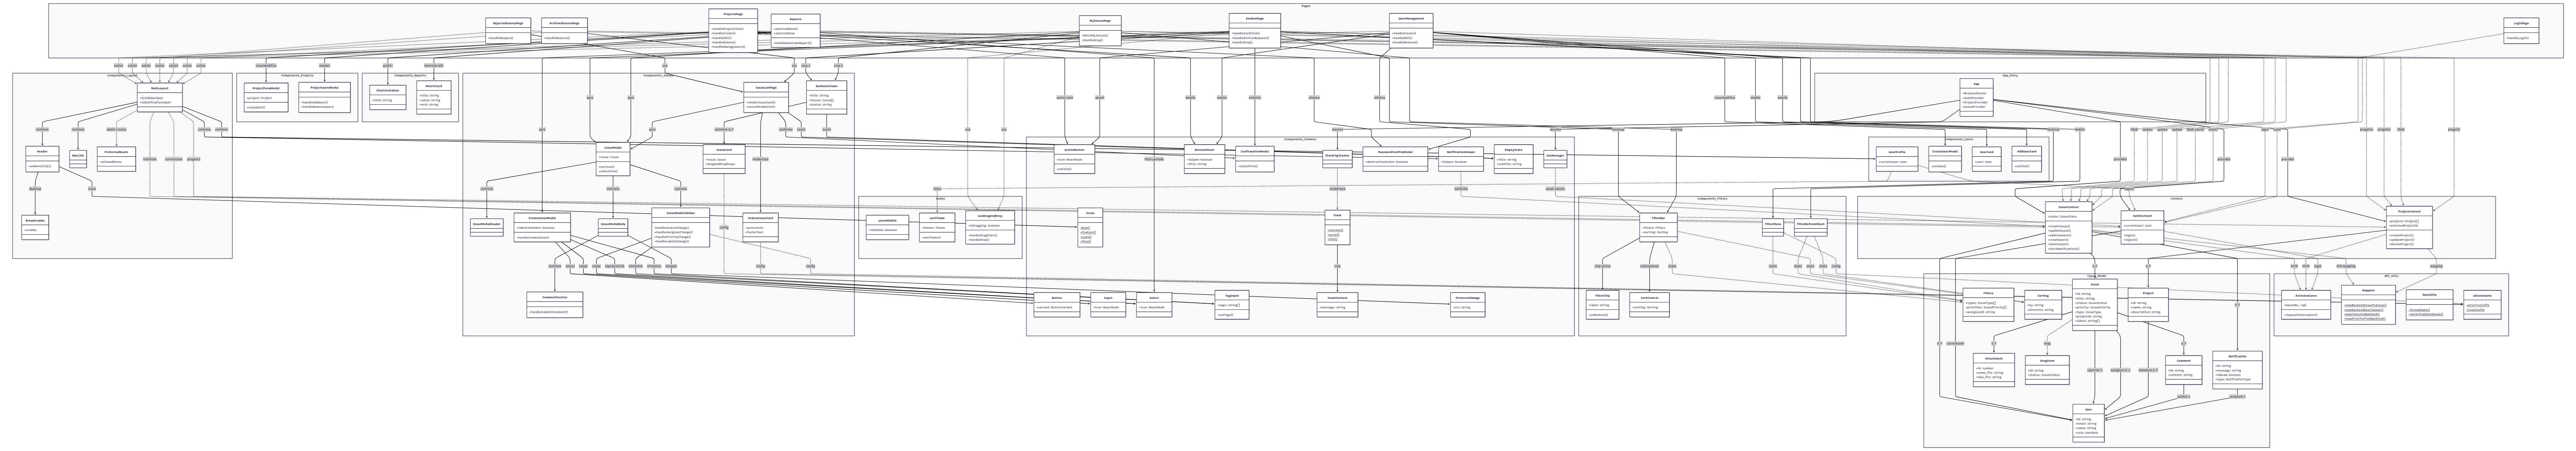
\includegraphics[width=1\textwidth]{ui_completo_bb26.png}
    \caption{Schema del front end}
\end{figure}

\newpage
\subsection{Scelte di design}

Il progetto BugBoard26 è stato strutturato per essere facile da mantenere e da estendere. Per fare ciò, sia nel backend che nel frontend abbiamo seguito i principi SOLID e alcuni design pattern fondamentali.

\subsubsection{Backend}

Il backend in Java e Spring Boot usa un'architettura a livelli (controller, service, repository, entity), in modo da tenere separate le diverse responsabilità e semplificare il collaudo delle singole parti.

\paragraph{Principio di Singola Responsabilità (SRP)}
Abbiamo diviso i compiti rigidamente: i controller gestiscono solo le chiamate HTTP, i service contengono tutta la logica di business e le conversioni tra entità e DTO, mentre i repository dialogano esclusivamente col database. Questo evita di avere file enormi che fanno troppe cose.

\paragraph{Dependency Inversion Principle (DIP)}
Spring gestisce l'iniezione delle dipendenze (Dependency Injection) tramite l'annotazione \texttt{@Autowired}. Questo significa che controller, service e repository non istanziano direttamente le classi da cui dipendono, ma ricevono i componenti pronti all'uso. In questo modo è molto più facile effettuare test usando dei mock.

\paragraph{Design pattern applicati nel backend}

\begin{itemize}
    \item \textbf{Singleton:} Spring gestisce i bean annotati con \texttt{@Service}, \texttt{@Repository} o \texttt{@RestController} creando un'unica istanza condivisa. Ad esempio, \texttt{SseService} usa una singola mappa per tenere traccia di tutti i client SSE connessi.

    \item \textbf{Builder:} Abbiamo sfruttato questo pattern sia per creare gli eventi passati via SSE tramite il metodo \texttt{SseEmitter.event()}, sia impostando la catena dei filtri HTTP in \texttt{WebSecurityConfig} con chiamate a cascata.

    \item \textbf{Adapter:} Il package \texttt{dto} converte il formato delle entità JPA in quello atteso dai client REST e viceversa. Così evitiamo di esporre la struttura del database direttamente verso l'esterno.

    \item \textbf{Observer:} Attraverso i Server-Sent Events, i client si collegano all'endpoint \texttt{/api/sse/subscribe/\{email\}} in attesa di novità. Il \texttt{SseService} fa da \textit{subject} avvisando i vari client quando ci sono aggiornamenti interessanti, come una nuova issue o un'assegnazione.

    \item \textbf{State:} Una issue può cambiare stato (aperta, chiusa, ecc.) usando i valori dell'enum \texttt{stato\_issue}. Il passaggio da uno stato all'altro viene preventivamente validato dal \texttt{IssueService} prima del salvataggio nel database.
\end{itemize}

\subsubsection{Frontend}

L'interfaccia React è stata divisa in componenti riutilizzabili. Sono raggruppati sia per area funzionale (come issues, projects, users) che per utilità comune (layout, filtri).

\paragraph{Principio di Singola Responsabilità (SRP)}
Anche qui, ogni componente fa una cosa sola. Ad esempio, \texttt{IssueCard} mostra i dati di base di una singola issue, \texttt{FilterBar} si occupa solo dei comandi di ricerca, e \texttt{StackingToaster} raccoglie gli avvisi a schermo. Lo stato globale dell'app è invece concentrato nei Context React.

\paragraph{Design pattern applicati nel frontend}

\begin{itemize}
    \item \textbf{Singleton:} In \texttt{api/axios.ts} c'è un'unica istanza di Axios già configurata con URL base e header predefiniti. In questo modo tutta l'app fa chiamate di rete partendo dalla stessa base.

    \item \textbf{Decorator:} Gli interceptor di Axios aggiungono l'header di autorizzazione in automatico a ogni richiesta senza toccare il codice di chi fa la chiamata. Allo stesso modo, il wrapper \texttt{ProtectedRoute} controlla i permessi di accesso prima di far vedere il vero contenuto della pagina.

    \item \textbf{Composite:} Molte interfacce derivano dall'unione di parti più piccole. Il popup \texttt{IssueModal}, ad esempio, è fatto mettendo insieme un header, un body, la sidebar laterale e la sezione dei commenti.

    \item \textbf{Observer:} Sfruttando i Context (\texttt{AuthContext}, \texttt{IssueContext}, \texttt{ProjectContext}), i componenti reagiscono al cambio dei dati centralizzati e si aggiornano da soli. Il componente \texttt{SseManager} ascolta il canale degli eventi dal backend e notifica le modifiche al resto dell'applicazione.

    \item \textbf{Builder:} Quando un utente compila un form o una modale per creare una issue, i dati vengono costruiti un pezzo alla volta nello stato del componente prima di formare il payload finale inviato al server.
\end{itemize}

